\documentclass[a4paper, 11pt]{article}

\usepackage{hyperref}
\voffset -0cm
\hoffset 0.0cm
\textheight 23cm
\textwidth 16cm
\topmargin 0.0cm
\oddsidemargin 0.0cm
\evensidemargin 0.0cm

\usepackage{epsfig}
\usepackage{setspace}
\usepackage{fancyheadings}
\usepackage{amsmath}
\usepackage{amssymb}
\usepackage{graphicx}
\usepackage{url}

\title{}
\author{}
\date{}

\begin{document}

\begin{center}
	\LARGE \textbf{TD12: Height maps and Mesh visualization}
\end{center}

\bigskip
\par In this practical work, the objective is to practice a bit with
triangular mesh data-structures and 3D visualization using
\texttt{DGtal}. The final objective is to render height maps as 3D
meshes with colorimetric information.

\section{Preliminaries}

Visualization will be performed by \texttt{DGtal}. If you use the
compiled library (``dcoeurjo'' account), the viewer is enabled by
default. If you use you own \texttt{DGtal} install, make sure that you
have compiled the library with \texttt{WITH\_QGLVIEWER} flag enables
(e.g. \texttt{cmake .. -DWITH\_QGLVIEWER=true}). You would need to
have Qt and QGLViewer installed in your system.

Please also checkout the last release of the \texttt{DGtalSkel} folder. The
file \texttt{image2mesh.cpp} gives examples of the \texttt{Viewer3D}
usage (please have a look to the C++ comments for details).

First, compile this example and when executing it, you should see an OpenGL
window with three triangles and two cubes.  For this TP, you just need
to know how to display triangles:
\begin{verbatim}
      Z3i::RealPoint p1(1.0,0.0,0.0),
        p2(0.0,1.0,0.0),
        p3(0.0,0.0,1.0);
      viewer.addTriangle(p1,p2,p3);
      viewer  << Viewer3D<>::updateDisplay;
\end{verbatim}


The idea is to construct a mesh from and image $I$ such that the mesh
vertices are given by 3D points $(i,j, I(i,j))$ for each point $(i,j)$
in the image domain.  As illustrated in Fig.~\ref{fig:image}, the mesh
is constructed from a regular pattern with alternate triangles with
respect to evenness of the y-coordinate for instance: $\{(i,j,I(i,j)),
(i+1,j,I(i+1,j)), (i,j+1,I(i,j+1))\}$ or $\{(i,j,I(i,j)),
(i+1,j-1,I(i+1,j-1)), (i+1,j,I(i+1,j))\}$

\begin{figure}[h]
  \begin{center}
    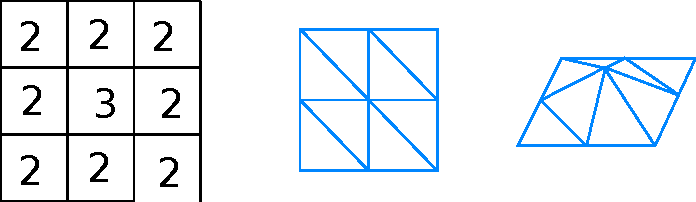
\includegraphics[width=10cm]{image2mesh}
  \end{center}
  \caption{Image to height map mesh.}
  \label{fig:image}
\end{figure}

Please note that \texttt{image2mesh.cpp} also contains a piece of code
to load a  PGM grayscale image.


\section{Mesh data-structure and visualization}

{\bf Question 1}  From a PGM image, construct a Face-Vertex data
structure: the Vertex vector contains all point coordinates and the
Face vector contains the faces (triple of vertex indices).


{\bf Question 2} Create a function which take in argument a mesh (the
two Face/Vertex  vectors) and send all triangles to a DGtal Viewer.

As an example, you can use height map of the Rhone (rhone1.pgm and
rhone3.pgm in the git repository):
 \begin{center}
    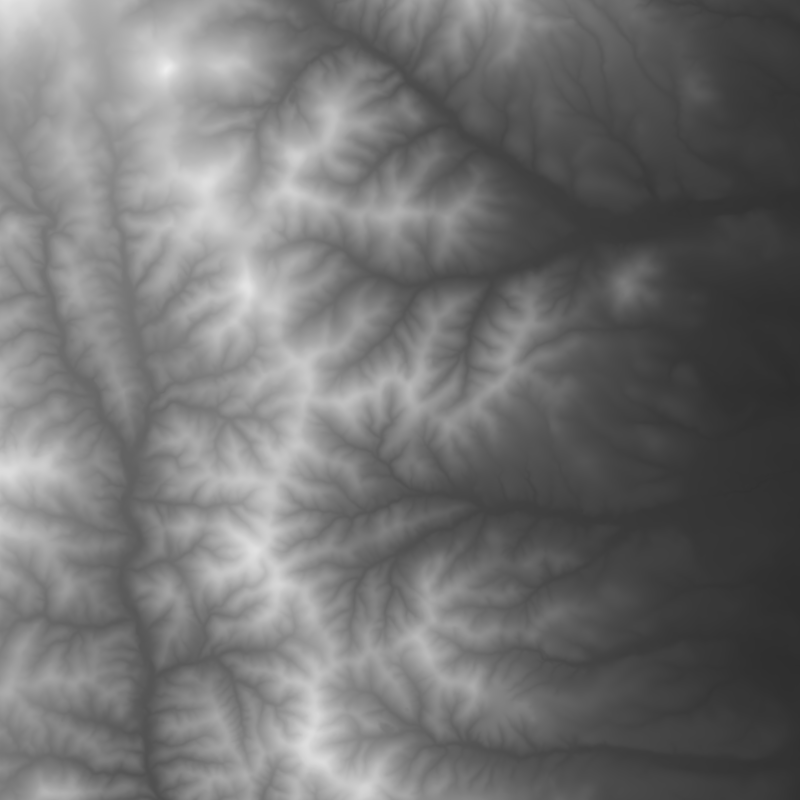
\includegraphics[width=6cm]{rhone1}
    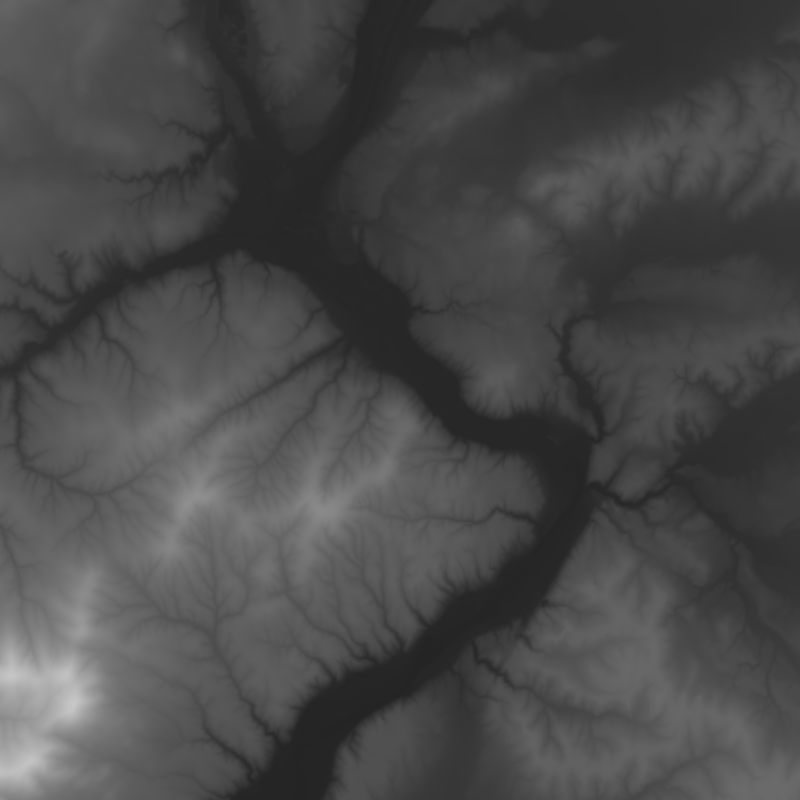
\includegraphics[width=6cm]{rhone3}
  \end{center}
If the images are to large, please consider using gimp to subsample them.
 


{\bf Question 3} Update the drawing function to change the color of
each triangle according to the mean height of the neighboring vertices
(using for instance a colormap from DGtal or you own function).



\section{Normal map rendering and curvature estimation}


{\bf Question 4} We would like now to see the normal map rendering of
the surface. Formally, if $\vec{n}$ is the normal vector to the
triangle, we want the colormap to follow the quantity $\vec{n}\cdot
(0,0,1)^t$ (scalar product between the normal and the z-axis.



{\bf Question 5} Curvature map: we would like now to color the mesh
from curvature information. Since the original data is a 2-dimensional
image, you can use a finite-difference approach to estimate the second
derivative of the image values. Use these values to control the color
of each triangle.




\end{document}
